\documentclass{beamer}
\mode<presentation>
  {
%   \usetheme{Berlin}
  %\usetheme{Dreuw}
  \usetheme{Dreuw}
  }
%  \usepackage{times}
  \usepackage{subfigure}
  \usepackage{relsize}
  \usepackage{tikz}
  \usepackage{listings}
  \usepackage{amsmath,amsthm, amssymb, latexsym}
 % \boldmath
  \renewcommand*{\thesubfigure}{}
%  \renewcommand{\figurename}{bvla}

\makeatletter
\providecommand\dotsum{\mathpalette\@dotted\sum \vphantom{\sum}}
\def\@dotted#1#2{\ooalign{\hfil$#1 \bullet $\hfil\cr\hfil$#1#2$\hfil\cr}}
\makeatother
\DeclareMathOperator*{\psum}{\mathchoice{\sum\!\!\!\!\!\!\!\bullet\ \ }{\sum\hspace{-2.2ex}\raisebox{0.2ex}{\scalebox{0.75}{$\bullet$}}\,\,}{\sum\!\!\!\!\!\!\!\bullet}{\sum\!\!\!\!\!\!\!\bullet}}
\DeclareMathOperator*{\psumm}{\mathchoice{\sum\!\!\!\!\!\!\!\bullet\ \ }{\sum\hspace{-2.6ex}\raisebox{0.15ex}{\scalebox{0.75}{$\bullet$}}\,\,}{\sum\!\!\!\!\!\!\!\bullet}{\sum\!\!\!\!\!\!\!\bullet}}

\DeclareMathOperator*{\pplus}{\oplus}
\newcommand{\dv}{\vec{t}}

  \usetikzlibrary{backgrounds}
\usetikzlibrary{automata}
\usetikzlibrary{arrows}
\usetikzlibrary{shapes}
\usetikzlibrary{decorations.pathmorphing}
\usetikzlibrary{fit}

\let\picturesize\Large

\def\clap#1{\hbox to 0pt{\hss#1\hss}}
\def\mathclap{\mathpalette\mathclapinternal}
\def\mathllap{\mathpalette\mathllapinternal}
\def\mathrlap{\mathpalette\mathrlapinternal}
\def\mathclapinternal#1#2{%
            \clap{$\mathsurround=0pt#1{#2}$}}
\def\mathllapinternal#1#2{%
            \llap{$\mathsurround=0pt#1{#2}$}}
\def\mathrlapinternal#1#2{%
            \rlap{$\mathsurround=0pt#1{#2}$}}


%%%%% TIKZ
\tikzstyle{every picture}=[line width=4pt]
\tikzstyle{ultra ultra thick}=[line width=2.5pt]
\tikzstyle{nodeSmall} = [state, minimum size=6mm, inner sep=0mm, fill=black, node distance=1.25cm]
\tikzstyle{state2}=[state, minimum size=7mm, inner sep=0.5mm]
\tikzstyle{teststate}=[state, minimum size=4mm, inner sep=0.5mm]
\tikzstyle{testleaf}=[minimum size=4mm, inner sep=0.5mm]
\tikzstyle{every loop}=[->]
\tikzstyle{onEdge}=[fill=white, pos=0.4]
\tikzstyle{testschuin}=[node distance=\testschuin]
\tikzstyle{test}=[node distance=\test, pos=0.4]
\tikzstyle{loopupper}=[in=67, out=113, loop]
\tikzstyle{lagerLabel}=[pos=0.68]
\tikzstyle{every scope}=[>=latex, node distance=\recht]
\tikzstyle{smallstate}=[state, minimum size=3mm, inner sep=0.5mm, fill=white, ultra ultra thick]
\tikzstyle{smallstate3}=[state, minimum size=3mm, inner sep=2mm, fill=white]
\tikzstyle{smallrectangle}=[state, rectangle, minimum size=3mm, inner sep=0.5cm, fill=white]
\tikzstyle{smallstate2}=[state, minimum size=5mm, inner sep=0.5mm, fill=white]
\tikzstyle{background rectangle}= [rounded corners, fill=yellow!20, draw=black, rounded corners=1ex]
\tikzstyle{oval} = [state, ellipse, minimum size=4mm, inner sep=0.5mm, node distance=1.5cm]
\tikzstyle{prob}=[->, decorate, decoration={snake,segment length=2mm, amplitude=.4mm,post length=1mm}]




\tikzstyle{loopleft}=[in=-176, out=-184, loop, swap]
\definecolor{greenish}{rgb}{0,0.5,0}
\tikzstyle{loopright}=[in=-10, out=10, loop, swap]
\tikzstyle{loopleft2}=[in=-171, out=-189, loop, swap]

\newlength{\testschuin}
\newlength{\test}
\newlength{\recht}
\setlength{\testschuin}{2.1213203435596425732025330863145cm}
\setlength{\test}{1.5cm}
\setlength{\recht}{1.7677669529663688110021109052621cm}
\newcommand{\back}{\picturesize \color{yellow!20}.}
\newcommand{\fail}{\bf \vphantom{p}fail\vphantom{f}}
\newcommand{\pass}{\bf \vphantom{p}pass\vphantom{f}}
%%%%%%%% TIKZ


  \usepackage[english]{babel}
  \usepackage[latin1]{inputenc}
%   \usepackage[textpos}
  \usepackage[absolute,overlay]{textpos}
  \usepackage[orientation=portrait,size=a0,scale=1.35,debug]{beamerposter}

  %%%%%%%%%%%%%%%%%%%%%%%%%%%%%%%%%%%%%%%%%%%%%%%%%%%%%%%%%%%%%%%%%%%%%%%%%%%%%%%%%5
  \graphicspath{{figures/}}

  \title[]{\Large Embedded System SImulator Generator}
  \author[]{\LARGE \textbf{
	Mark Florisson,
	Ruud Harmsen,
	Wilfried van Asten,
	Ewoud Kohl van Wijngaarden
  }}

  \institute{\Large \vfill {Ontwerpproject (192199109) -- Faculty of Electrical Engineering -- University of Twente} }
  \date{}

  \begin{document}
  \begin{frame}{}

\vspace{-1cm}
% Eerste rij
\begin{columns}[t]
\begin{column}{.02\linewidth}\end{column}
\begin{column}{.97\linewidth}\begin{block}{\large \smash{Introduction}\vphantom{Introduction}}
\end{block}

\end{column}
\begin{column}{.02\linewidth}\end{column}
\end{columns}

\vskip0.01\linewidth
%\vfill

% Tweede rij
\begin{columns}[t]
\begin{column}{.02\linewidth}\end{column}
\begin{column}{.475\linewidth}\begin{block}{\large \smash{Example Specficication}\vphantom{Example Code}}

\tiny {  
\lstset{
numbers=left,                   % where to put the line-numbers
numberstyle=\tiny,      % the size of the fonts that are used for the line-numbers
stepnumber=1,
xleftmargin=25pt,
backgroundcolor=\color{lightgray},
frame=single
}

Specify the microcontroller as type 'demo'.
\begin{lstlisting}
demo {
\end{lstlisting}

Define general parameters.
\begin{lstlisting}[name=demo.dmo]
	parameters {
		gprs 2+5;
		opcode-size 16;
		clock 1;
		endianness little;
	}
\end{lstlisting}

Define register offsets.
\begin{lstlisting}[name=demo.dmo]
	registers {
		SREG	= 0x5F;
		PC	= 0x462;
		SP	= 0x5D;
	}
\end{lstlisting}

Define memory mappings.
\begin{lstlisting}[name=demo.dmo]
	maps {
		chunk		(0, 0xFFFFFFF);
		register	(0, 0x20);
		io		(0x20, 0x60);
		ram		(0, 0x461);
		rom		(0x464, 0xFFFFFF);
		print		(0x3b, 0x3c);
	}

\end{lstlisting}

Define instructions
\begin{lstlisting}[name=demo.dmo]
	instructions {
		noop "0000 0000 0000 0000" {
			PC = PC + 1;
		}

		/* Load an I/O Location to Register */
		in "1011 0AAd dddd AAAA" Rd, A {
			Rd = io($A);

			PC = PC + 1;
		}

		jmp "1001 010k kkkk 110k", "kkkk kkkk kkkk kkkk" k {
			PC = $k;
		}
	}
}  
\end{lstlisting}

}

\end{block}
\end{column}
\begin{column}{.01\linewidth}\end{column}
\begin{column}{.475\linewidth}\begin{block}{\large \smash{Goals}\vphantom{Example}}
\end{block}

\end{column}
\begin{column}{.02\linewidth}\end{column}
\end{columns}

%\vfill
\vskip0.01\linewidth

% Derde rij
\begin{columns}[t]
\begin{column}{.02\linewidth}\end{column}
\begin{column}{.475\linewidth}\begin{block}{\large \smash{Future use}\vphantom{Future}}
\begin{itemize}
    \item Embedded System Toolchain Development
    \item Code Testing \& Debugging
    \item Hardware Prototyping
    \item Model Checking
\end{itemize}
%\begin{wrapfigure}{r}{\textwidth}
%\infobox{Eclipse Debugging}{
%    \begin{figure}[t]
    \begin{figure}[!htb]
        \vspace{-100pt}
        \hspace{350pt}
        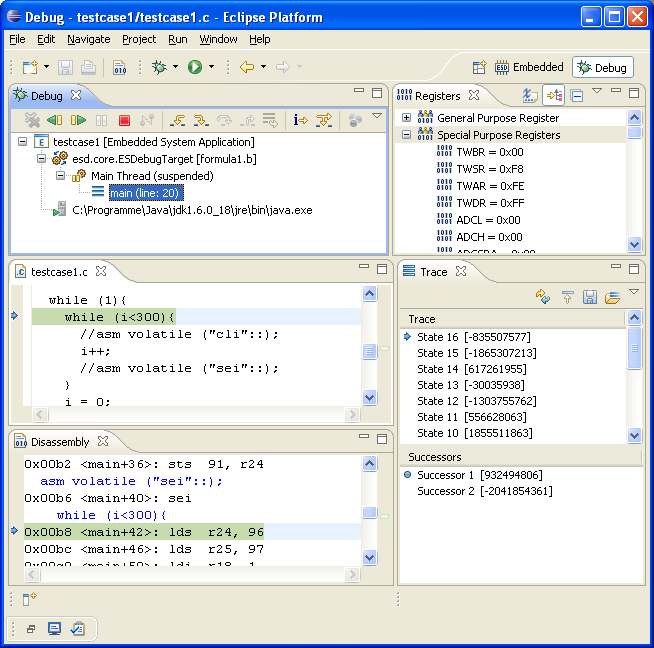
\includegraphics{figures/overview.jpg}
    \end{figure}
%}
%\end{wrapfigure}
\end{block}
\end{column}
\begin{column}{.01\linewidth}\end{column}
\begin{column}{0.475\linewidth}

\setbeamertemplate{block begin}{
  \vskip.75ex
  \begin{beamercolorbox}[rounded=true,shadow=true,leftskip=1cm,colsep*=.75ex]{block title}%
    \usebeamerfont*{block title}\insertblocktitle
  \end{beamercolorbox}%
  {\ifbeamercolorempty[bg]{block body}{}{\nointerlineskip\vskip-0.5pt}}%
  \usebeamerfont{block body}%
  \begin{beamercolorbox}[ht=17.45cm, rounded=true,shadow=true,colsep*=.75ex,sep=.75ex, vmode]{block body}%
    \ifbeamercolorempty[bg]{block body}{\vskip-.25ex}{\vskip-.75ex}\vbox{}%
    \begin{adjustwidth}{0.8cm}{0.4cm}
  }
  \setbeamertemplate{block end}{
  \end{adjustwidth}
  \end{beamercolorbox}
}

\begin{block}{\large \smash{7. Results and Future Work} \vphantom{Introduction}}
\textbf{Results:}
\begin{adjustwidth}{0.5cm}{0.5cm}
\begin{itemize}
\item \ We developed the \alert{process algebra prCRL}, incorporating both \alert{data} and 
\item[] \ \alert{probability}.
\item \ We defined a \alert{linear format for prCRL}, the \alert{LPPE}, providing the starting 
\item[] \ point for effective symbolic optimisations and easy state space generation.
\item \ We provided a \alert{linearisation algorithm} to transform prCRL  specifications 
\item[]\  to their corresponding LPPE, proved it \alert{correct}, and \alert{implemented} it.
\end{itemize}
\end{adjustwidth}

\noindent\\ \phantom{x}\noindent\\

\textbf{Future work:}
\begin{adjustwidth}{0.5cm}{0.5cm}
\begin{itemize}
\item \ Applying existing optimisation techniques, such as \alert{constant elimination},
\item[] \  \alert{liveness analysis} and \alert{confluence reduction}, to LPPEs.
\end{itemize}
\end{adjustwidth}
\vskip10pt
\end{block}

\vskip0.02\linewidth

\setbeamertemplate{block begin}{
  \vskip.75ex
  \begin{beamercolorbox}[rounded=true,shadow=true,leftskip=1cm,colsep*=.75ex]{block title}%
    \usebeamerfont*{block title}\insertblocktitle
  \end{beamercolorbox}%
  {\ifbeamercolorempty[bg]{block body}{}{\nointerlineskip\vskip-0.5pt}}%
  \usebeamerfont{block body}%
  \begin{beamercolorbox}[rounded=true,shadow=true,colsep*=.75ex,sep=.75ex, vmode]{block body}%
    \ifbeamercolorempty[bg]{block body}{\vskip-.25ex}{\vskip-.75ex}\vbox{}%
    \begin{adjustwidth}{0.8cm}{0.4cm}
  }
  \setbeamertemplate{block end}{
  \end{adjustwidth}
  \end{beamercolorbox}
}

%\vskip45pt

\begin{block}{\large \smash{8. Acknowledgments} \vphantom{Introduction}}
This research is supported by NWO under grant 612.063.817 (SYRUP) 
and grant Dn 63-257 (ROCKS), and by the European Union under FP7-ICT-2007-1 
grant 214755 (QUASIMODO).
\end{block}
\end{column}
\begin{column}{.02\linewidth}\end{column}
\end{columns}

%\vfill

\end{frame}
\end{document}
